\documentclass{standalone}
\usepackage[calc]{picture}
\usepackage{graphicx,transparent,color,amsmath,amssymb,amsfonts,tikz}
\graphicspath{Fig_SIM_subfigs}
\setlength{\unitlength}{1in}

\usepackage{helvet}
\renewcommand{\familydefault}{\sfdefault}
\begin{document}


\begin{picture}(11.1, 11.6)(-2.95,-8.9)
% ground truth 
\put(-1.4, 1.1){\includegraphics[height=1.05in, width=9.4in]{Fig_SIM_subfigs/example_temporal_true.pdf}}
\put(-2.3, 1.15){\includegraphics[height=1in]{Fig_SIM_subfigs/example_spatial_true.pdf}}
\linethickness{0.02in} \put(-2.35, 1.1){\color{black}\line(1,0){10}}
\linethickness{0.02in} \put(-2.35,1.1){\color{black}\line(0,1){1.1}}
\linethickness{0.02in} \put(7.65, 1.1){\color{black}\line(0,1){1.1}}
\linethickness{0.02in} \put(-2.35, 2.2){\color{black}\line(1,0){10}}
\put(-2.6, 1.4){\Large\rotatebox{90}{{Truth}}}

% % PCA/ICA neuron
\put(-1.4, -0.05){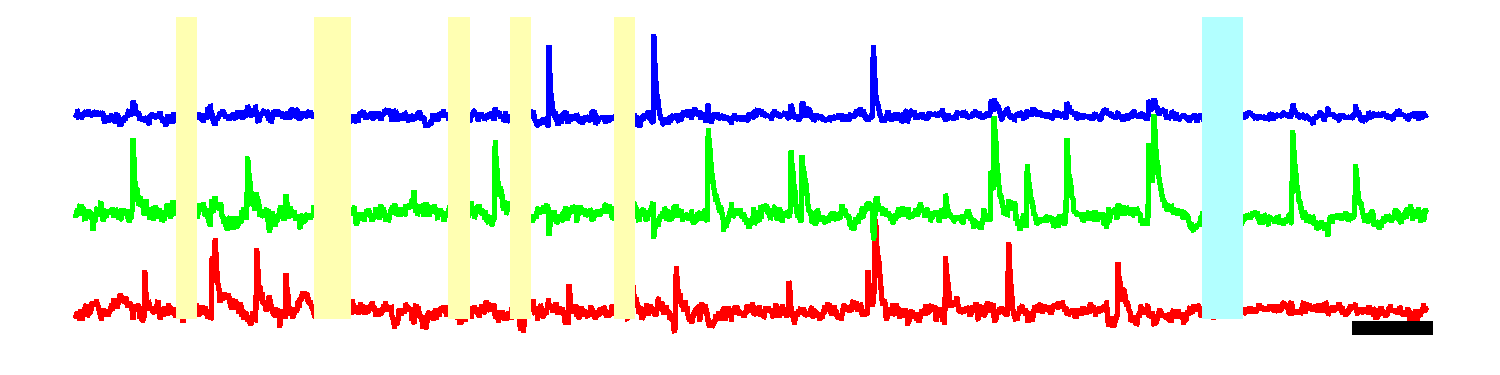
\includegraphics[height=1.05in, width=9.4in]{Fig_SIM_subfigs/example_temporal_ica.pdf}}
\put(-2.3, 0.0){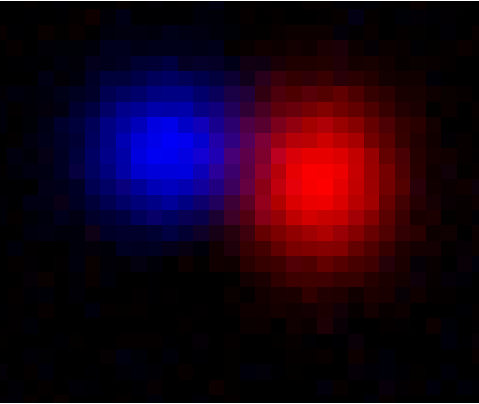
\includegraphics[height=1in]{Fig_SIM_subfigs/example_spatial_ica.pdf}}
\linethickness{0.02in} \put(-2.35, -0.05){\color{black}\line(1,0){10}}
\linethickness{0.02in} \put(-2.35,-0.05){\color{black}\line(0,1){1.1}}
\linethickness{0.02in} \put(7.65, -0.05){\color{black}\line(0,1){1.1}}
\linethickness{0.02in} \put(-2.35,1.05){\color{black}\line(1,0){10}}
\put(-2.6, 0.1){\Large\rotatebox{90}{{PCA/ICA}}}

% CNMF neuron 
\put(-1.4, -1.2){\includegraphics[height=1.05in, width=9.4in]{Fig_SIM_subfigs/example_temporal_cnmf.pdf}}
\put(-2.3, -1.15){\includegraphics[height=1in]{Fig_SIM_subfigs/example_spatial_cnmf.pdf}}
\linethickness{0.02in} \put(-2.35,-1.2){\color{black}\line(1,0){10}}
\linethickness{0.02in} \put(-2.35,-1.2){\color{black}\line(0,1){1.1}}
\linethickness{0.02in} \put(7.65,-1.2){\color{black}\line(0,1){1.1}}
\linethickness{0.02in} \put(-2.35,-0.1){\color{black}\line(1,0){10}}
\put(-2.6, -0.95){\Large\rotatebox{90}{{CNMF}}}

% CNMF-E neuron 
\put(-1.4, -2.35){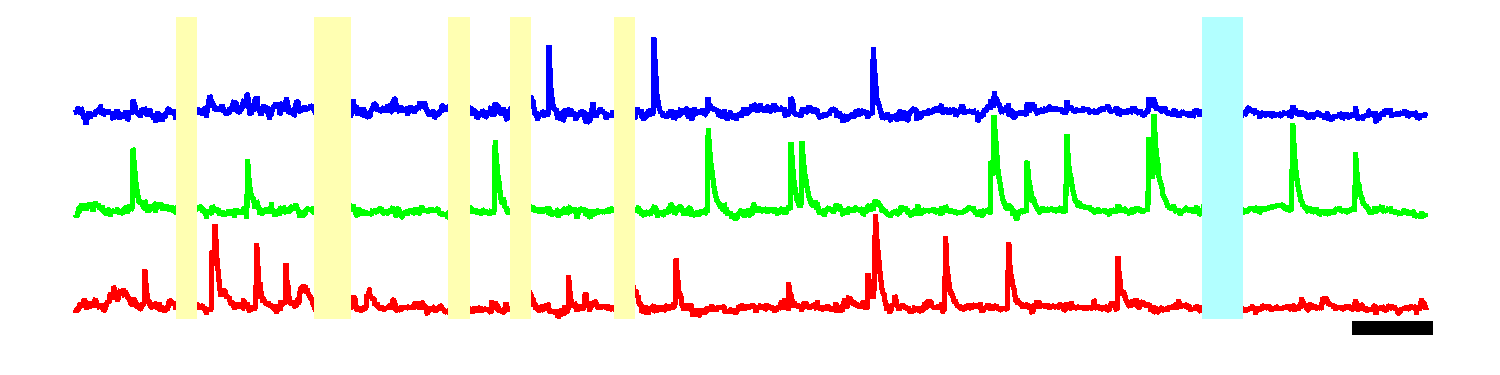
\includegraphics[height=1.1in, width=9.4in]{Fig_SIM_subfigs/example_temporal_cnmfe.pdf}}
\put(-2.3, -2.3){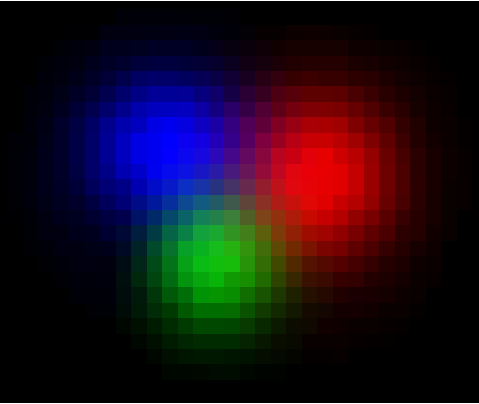
\includegraphics[height=1in]{Fig_SIM_subfigs/example_spatial_cnmfe.pdf}}
\linethickness{0.02in} \put(-2.35,-2.35){\color{black}\line(1,0){10}}
\linethickness{0.02in} \put(-2.35,-2.35){\color{black}\line(0,1){1.1}}
\linethickness{0.02in} \put(7.65,-2.35){\color{black}\line(0,1){1.1}}
\linethickness{0.02in} \put(-2.35,-1.25){\color{black}\line(1,0){10}}
\put(-2.6, -2.2){\Large\rotatebox{90}{{CNMF-E}}}

\put(-2.75, 2.25){\Large\textbf{A}}
\put(2., 2.3){\Large{Example neurons}}

\put(-3.1, -5.9){\includegraphics[height=3.2in]{./Fig_SIM_subfigs/RSS.png}}
\put(-2.85, -2.75){\Large\textbf{B}}
\put(-1.6, -2.7){\Large{RSS during the iterations}}

\put(1.25,-5.899){\includegraphics[height=3.15in]{Fig_SIM_subfigs/example_sim_similarity_fisher.pdf}}
\put(1.2, -2.75){\Large\textbf{C}}
\put(2.0, -2.7){\Large{Similarities with the truth}}

\put(4.65, -5.899){\includegraphics[height=3.1in]{Fig_SIM_subfigs/example_sim_correlation_separate.png}}
\put(4.5, -2.75){\Large\textbf{D}}
\put(5.4, -2.7){\Large{Pairwise correlations}}

\put(2.25,-8.8){\includegraphics[height=2.65in]{Fig_SIM_subfigs/noise_temporal_similarity.pdf}}
\put(2.5, -6.1){\Large\textbf{G}}


\put(-0.3,-8.8){\includegraphics[height=2.65in]{Fig_SIM_subfigs/noise_spatial_similarity.pdf}}
\put(-0.25, -6.1){\Large\textbf{F}}


\put(-2.9,-8.8){\includegraphics[height=2.65in]{Fig_SIM_subfigs/false_negatives.pdf}}
\put(-2.85, -6.1){\Large\textbf{E}}


\put(4.9,-8.5){\includegraphics[height=2.5in, width=3in]{Fig_SIM_subfigs/noise_traces.pdf}}
\put(4.9, -6.1){\Large\textbf{H}}

% \put(-0.1,-11.25){\includegraphics[height=2.2in]{Fig_SIM_subfigs/similarity_corr.pdf}}
% \put(-0.1, -8.95){\Large\textbf{I}}
% \put(1.55, -8.9){Extraction accuracy}

% \put(4.35,-10.85){\includegraphics[height=2.0in]{Fig_SIM_subfigs/example_corr.pdf}}
% \put(4.25, -8.95){\Large\textbf{J}}
% \put(5.5, -8.9){Example simulation}
% % \put(3.4, -3.65){\textbf{I}}
% \put(4.27, -9.15){(i)}
% \put(4.25, -9.6){(ii)}
% \put(4.25, -10.05){(iii)}
% \put(4.25, -10.5){(iv)}

% \put(4.5, -3.65){\footnotesize Example simulation}

\end{picture}
\end{document}
